\documentclass{standalone}

\usepackage{tikz,pgf}
\usetikzlibrary{arrows}

\newcommand{\file}[1]{\begin{tikzpicture}
	\foreach \y in {0.15,0.3,...,1.20}{
		\draw[line width=0.5mm,gray] (0.1,\y) -- (0.9,\y);
	}
	\path[fill=white] (0.75,1.25) -- (0.75,1) -- (1,1);
	\path[draw] (0.75,1.25) -- (0,1.25) -- (0,0) -- (1,0) -- (1,1) -- (0.75,1.25) -- (0.75,1) -- (1,1);
	\node[scale=0.8,fill=white,inner sep=0mm] at (0.5,-0.25) {#1};
\end{tikzpicture}}

\begin{document}
	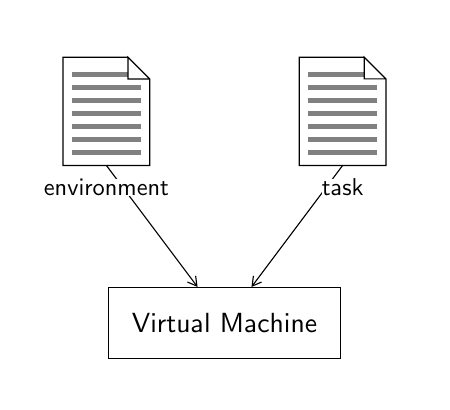
\begin{tikzpicture}[font=\sf,component/.style={draw,shape=rectangle, inner sep=3mm,minimum height=0.9cm}]
		\useasboundingbox (-2.5,3.75) rectangle (2.5,-0.75);
		%%%
		\node[component] (vm) at (0,0) {Virtual Machine};
		\draw[-angle 60] (-1.5,2) -- (vm);
		\draw[-angle 60] (1.5,2) -- (vm);
		\node[scale=1.1] at (-1.5,2.5) {\file{environment}};
		\node[scale=1.1] at (1.5,2.5) {\file{task}};
		%%%
	\end{tikzpicture}
\end{document}